% Offizielle Beispieldatei für beamer-Vorlage aus tubslatex Version 0.3beta2
\documentclass[fleqn,11pt,aspectratio=43]{beamer}

\usepackage[ngerman]{babel}
\usepackage[utf8x]{inputenc}
\usepackage{svg}
\usepackage{pdfpages}
\usepackage{graphicx}

\newcommand{\topbottombraced}[2]{%
  \raise.5ex\vtop{
    \vbox{%
      \hbox{$\left\{\begin{tabular}{@{}l@{}}#1\end{tabular}\right\}$}
      \vskip1pt
    }
    \vbox{%
      \vskip1pt
      \hbox{$\left\{\begin{tabular}{@{}l@{}}#2\end{tabular}\right\}$}
    }
  }%
}
\usetheme[%
  %nexus,%        Nexus Fonts benutzen
  %lnum,%         Versalziffern verwenden
  %cmyk,%<rgbprint>,          Auswahl des Farbmodells
  blue,%<orange/green/violet> Auswahl des Sekundärfarbklangs
  dark,%<light,medium>        Auswahl der Helligkeit
  %colorhead,%    Farbig hinterlegte Kopfleiste
  %colorfoot,%    Farbig hinterlegt Fußleiste auf Titelseite
  colorblocks,%   Blöcke Farbig hinterlegen
  %nopagenum,%    Keine Seitennumer in Fußzeile
  %nodate,%       Kein Datum in Fußleiste
  tocinheader,%   Inhaltsverzeichnis in Kopfleiste
  %tinytocinheader,% kleines Kopfleisten-Inhaltsverzeichnis
  %widetoc,%      breites Kopfleisten-Inhaltsverzeichnis
  %narrowtoc,%    schmales Kopfleisten-Inhaltsverzeichnis
  %nosubsectionsinheader,%  Keine subsections im Kopfleisten-Inhaltsverzeichnis
  %nologoinfoot,% Kein Logo im Fußbereich darstellen
  ]{tubs}

% Titelseite
\title{Entwurf einer adaptiven Regelung für Kältekreisläufe}
\subtitle{auf Basis des natürlichen Kältemittels CO\textsubscript{2}}
\author{Carl Julius Martensen}
% Titelgrafik, automatisch beschnitten, Weitere Optionen: <scaled/cropx/cropy>
% \titlegraphic[scaled]{\includegraphics{infozentrum.jpg}}
\titlegraphic[cropped]{\includegraphics{title}}

% Logo, dass auf Titelseiten oben rechts und auf Inthaltsseiten unten rechts
% dargestellt wird. Es wird jeweils automatisch skliert
\logo{\includegraphics{ift_4C.pdf}}
%\logo{Institut für Unkreativität\\und Schreibschwäche}

\begin{document}

\begin{frame}[plain]
\titlepage
\end{frame}

\section*{Inhalt}
\begin{frame}
\tableofcontents
\end{frame}

\section{Motivation und Übersicht}

\begin{frame}{Motivation}
  \begin{columns}[onlytextwidth]
    \column{0.45\textwidth}
	\begin{exampleblock}{Prozessregelung}
		\begin{itemize}
			\item Einfache Reglerstrukturen
			\item Optimale Arbeitspunkte
			\item Reglerparametrierung nicht optimal
		\end{itemize}
	\end{exampleblock}
	\begin{alertblock}{Lösung}
	\begin{itemize}
		\item Autotuning
		\item Robustheit
		\item Mehrgrößenregelung
	\end{itemize}
	\end{alertblock}
    \column{0.45\textwidth}
    \begin{figure}\centering
    \resizebox{\textwidth}{!}{\includesvg{../Graphics/Working_Point_Uncertainty}}
    \end{figure}
  \end{columns}
\end{frame}

%\begin{frame}{Motivation}
%Hier einmal die Motivation aus Sicht der Thermodynamik:
%- Autotuning bringt Vorteile
%-> MPC berechnet Optimale Arbeitspunkte
%-> Optimale Arbeitspunkte nahe am Rand des Naßdampfgebietes
%-> Reale Umsetzung der Arbeitspunkte hängt stark von Führungs- und Störungsverhalten ab 
%\end{frame}


%\begin{frame}{Vorgehen}
%- Recherche -> Mehrgrößenregler, Vorgehen, Maße etc
%- Algorithmus Entwicklung: Matlab und Python
%- Übergang zu Simulationsstudien: Umsetzung in Modelica, Simulation mit Python und MoBa
%- Übergang auf das Physikalische System
%\end{frame}

\begin{frame}{Strategie}

\begin{columns}[onlytextwidth]
\column{0.45\textwidth}
\textbf{Arbeitsschritte}\\
\begin{alertblock}{Eingrößenregelung}
Identifikation \\
Reglerparameter
\end{alertblock}


\begin{alertblock}{Mehrgrößenregelung}
Paarungen \\
Entkopplung \\
Detuning
\end{alertblock}

\column{0.45\textwidth}
\textbf{Umsetzung}\\
\begin{exampleblock}{Eingrößenregelung}
First Order Time Delay \\
AMIGO Algorithmus
\end{exampleblock}

\begin{exampleblock}{Mehrgrößenregelung}
Relative Gain Array (RGA)\\
Splitter \\
AMIGO Detuning
\end{exampleblock}

\end{columns}
\begin{center}
Modularer Aufbau
\end{center}
\end{frame}

\begin{frame}{Werkzeugkette}
\begin{table}[h!]
\begin{center}
\begin{tabular}{l r}
\raisebox{-0.5\totalheight}{\includegraphics[width = 0.2\textwidth]{Modelica.png} }& Systemmodellierung, Implementierung der Regler\\ & \\
\raisebox{-.4\totalheight}{\includegraphics[width = 0.2\textwidth]{fmi-logo.png}} & Schnittstelle zwischen Modelica und Python  \\ & \\
\raisebox{-.5\totalheight}{\includegraphics[width = 0.2\textwidth]{python-programming-assignment-help.png}} & Algorithmen, Simulation, Auswertung \\ & \\
\raisebox{-.5\totalheight}{\includegraphics[width = 0.2\textwidth]{MATLAB-Logo.png}} & Algorithmen, Simulation, Auswertung  \\
\end{tabular}
\end{center}
\end{table}
\end{frame}

%- Identifikation im Arbeitspunk / Modellbildung
%- Dezentrale Regler / Reglerauslegung
%- Erweitern der Reglerstruktur um Störungen
%- Detuning


\section{Eingrößenregelung}

\begin{frame}{Modellbildung}
\begin{columns}[onlytextwidth]
    \column{0.45\textwidth}
    	\resizebox{\columnwidth}{!}{\includesvg{../Graphics/Streckenmodell}}
    \column{0.45\textwidth}
	\begin{alertblock}{Problem}
		Dynamische Charakterisierung des Prozess für Autotuning ist notwendig.
	\end{alertblock}
	\begin{exampleblock}{Randbedingungen}
		\begin{itemize}
			\item Modell variiert stark
			\item Modell hochparametriert
			\item Reglerstruktur starr
			\item Reglerstruktur niedrig parametriert
		\end{itemize}
	\end{exampleblock}
  \end{columns}
\end{frame}

\begin{frame}{First Order Time Delay}
\begin{columns}[onlytextwidth]
\column{0.45\textwidth}
	\centering
	\resizebox{\columnwidth}{!}{\includesvg{../Graphics/FOTD_Identification2}}
\column{0.45\textwidth}
	\begin{exampleblock}{First Order Time Delay}
	Approximation des realen Übertragungsverhaltens durch ein Näherungsmodell
	\begin{itemize}
		\item Statische Verstärkung fehlerfrei
		\item Dominantes Verhalten erster Ordnung
		\item Approximation höherer Ordnungen durch Laufzeit
	\end{itemize}
	\end{exampleblock}
\end{columns}
\end{frame}

\begin{frame}{Beispiel einer Charakterisierung}
\centering\resizebox{\textwidth}{!}{\includesvg{../Graphics/FOTD_Identification_BIG}}
\end{frame}


%\begin{frame}{Approximation Hoher Ordnungen}
%\centering\resizebox{\textwidth}{!}{\includesvg{../Graphics/SISO_Robustness_Study_NormalizedTime}}
%\end{frame}

%\begin{frame}{Identifikation}%
%Einmal am Flächenbeispiel das vorge%hen zeigen.%
%Hier sogar Simulationsdaten nehmen!%
%Kurz auf Aströms Relay verweisen, aber anmerken, dass Arbeitspunkte sehr nahe am Phasenrand sind und daher ein schwingendes %Verfahren nicht geeignet ist.
%\end{frame}


%\begin{frame}{PI/PID Regler}%
%		\begin{exampleblock}{PI/PID Regler}%
%			Gibt ein \textbf{gewichtetes} Ausgangssignal auf Grundlage des% %zeitlichen Signalverlaufes von Sollwert $y_R$ und Istwert $y$ %zurück. 
%		\end{exampleblock}
%
%		\begin{exampleblock}{AMIGO Algorithmus}%
%			Gibt die notwendigen \textbf{Wichtungen} auf Grundlage der %Modellparameter eines FOTD zurück. 
%		\end{exampleblock}
%
%		\begin{alertblock}{Detuning}
%			\textbf{Reduziert} die Wichtungen . Der Regler wird langsamer.
%		\end{alertblock}
%
%		\begin{alertblock}{Setpoint-Weight}%
%			Wichtet Soll- und Istwert \textbf{einzeln}. Der Regler wird %langsamer.
%		\end{alertblock}
%\end{frame}
%
%\begin{frame}{Robustheit}
%\centering
%\resizebox{\textwidth}{!}{\includesvg{../Graphics/Maximum_Sensitivity}}
%\end{frame}
%
\begin{frame}[plain]{Robustheitsstudie}
\centering\resizebox{.8\textwidth}{!}{\includesvg{../Graphics/SISO_Robustness_Study}}
\end{frame}


\begin{frame}{Zwischenstand}

\begin{columns}[onlytextwidth]
\column{0.45\textwidth}
\begin{alertblock}{Eingrößenregelung \Huge{\checkmark}}
Identifikation \\
Reglerparameter
\end{alertblock}


\begin{alertblock}{Mehrgrößenregelung}
Paarungen \\
Entkopplung \\
Detuning
\end{alertblock}

\column{0.45\textwidth}
\begin{exampleblock}{Eingrößenregelung \Huge{\checkmark}}
First Order Time Delay \\
AMIGO Algorithmus
\end{exampleblock}

\begin{exampleblock}{Mehrgrößenregelung}
Relative Gain Array \\
Splitter \\
AMIGO Detuning
\end{exampleblock}

\end{columns}
\end{frame}

\section{Mehrgrößenregelung}

\begin{frame}{Systemdarstellung}
\begin{columns}[onlytextwidth]
\column{0.45\textwidth}
	\centering \resizebox{\textwidth}{!}{\includesvg{Kreislauf}}
\column{0.5\textwidth}
	\centering \resizebox{\textwidth}{!}{\includesvg{Cycle}}
\end{columns}
\end{frame}

\begin{frame}{Dezentrale Regelstruktur}
\begin{figure}\center
\includesvg[width = \linewidth]{control_standard}
\end{figure}
\end{frame}

\begin{frame}{Reale Regelstruktur}
\includesvg[width = \linewidth]{control_standard_coupling}
\end{frame}

\begin{frame}{Kopplungseffekte}
\resizebox{\textwidth}{!}{\includesvg{Identification_Example}}
\end{frame}

\begin{frame}{Entkopplung}
\includesvg[width = \linewidth]{control_standard_splitter}
\end{frame}

\begin{frame}{Sollwertänderung}
\centering
\resizebox{\textwidth}{!}{\includesvg{DecouplingExample}}
\end{frame}

\begin{frame}{Störgrößeneinfluss}
\centering
\resizebox{\textwidth}{!}{\includesvg{DisturbanceRejectionExample}}
\end{frame}


\section{Resumee und Ausblick}

\begin{frame}{Resumee}
\begin{columns}[onlytextwidth]
\column{0.45\textwidth}
\begin{exampleblock}{Ergebnisse}
\begin{itemize}
	\item Robuster Mehrgrößenregler
	\item Erhöhung der Positioniergenauigkeit
	\item Reduzierung der Störgrößeneinflüsse
\end{itemize}
\end{exampleblock}
\column{0.45\textwidth}

\begin{exampleblock}{Masterarbeit}
\begin{itemize}
	\item Diskussion der Algorithmen
	\item Robustheitsnachweise
	\item Theoretische Beispiele
	\item Simulative Studien
\end{itemize}
\end{exampleblock}
\end{columns}
\end{frame}

\begin{frame}{Ausblick}
\begin{exampleblock}{Erweiterung der Untersuchung}
\begin{itemize}
	\item Erweiterung um weitere Stellgrößen
	\item Simulative Studien mit Fokus auf energetische Vorteile
	\item Untersuchung der Identifizierungsprozedur
	\item Erweiterung auf Sliding-Mode
\end{itemize}
\end{exampleblock}
\begin{alertblock}{Nachweis am Prüfstand}
Durchführung experimenteller Studien am Prüfstand
\end{alertblock}
\end{frame}

\end{document}
